%\documentclass{article}
\documentclass{scrartcl}
\usepackage{titlesec}
\usepackage{enumitem}
%\usepackage{array,booktabs,arydshln,xcolor}
\usepackage{oesch}
\usepackage{graphicx}
\usepackage{caption}
\usepackage{float}

\graphicspath{ {images/} }

\setkomafont{disposition}{\normalfont\bfseries}


\setcounter{secnumdepth}{4}

\titleformat{\paragraph}
{\normalfont\normalsize\bfseries}{\theparagraph}{1em}{}
\titlespacing*{\paragraph}
{0pt}{3.25ex plus 1ex minus .2ex}{1.5ex plus .2ex}
\begin{document}
\title{Software Configuration Management Plan}
\subtitle{Avian Limited - Java Air}
\author{Amy Erxleben}

\maketitle
\newpage
\subsection*{Approvals}

\begin{center}
\begin{tabular}{|  l | c | r | }
\hline
  \textbf{Title} & \textbf{Signature} & \textbf{Date} \\ \hline
  Integration Engineer &  \oeschfamily Amy Erxleben & 10/03/16 \\ \hline
  Integration Engineer & \oeschfamily Amy Erxleben & 10/05/16 \\ \hline
  Integration Engineer & \oeschfamily Amy Erxleben & 11/04/16 \\ \hline
\end{tabular}
\end{center}

\subsection*{Revision History}

\begin{center}
\begin{tabular}{| l | l | p{10cm} | l |}
\hline
\textbf{Version} & \textbf{Author} & \textbf{Modifications} & \textbf{Date} \\ \hline
0.1.0 & Erxleben & Created first draft  & 10/01/16 \\ \hline
0.2.0 & Erxleben & Added sections ``Approvals'', ``Revision History'', and ``Annex A'', added content to sections 3.2.2.1-3.2.4 & 10/03/16 \\ \hline
1.0.0 & Erxleben & addded content to sections 3.3.2.1, 3.4, 3.6.  Updated content in section 3.2.2.1 \& 3.3.6, modified format of Approvals and Revision History & 10/05/16 \\ \hline
2.0.0 & Erxleben & sections 3.3.2.1 modified, Added Annex A, backup plan & 10/31/16\\ \hline
2.1.0 & Erxleben & updated sections 3.2.3 and 3.3.2.1 &11/04/16 \\ \hline
2.1.1 & Erxleben & corrected typos & 11/07/16 \\ \hline
\end{tabular}
\end{center}
\newpage

\setcounter{secnumdepth}{4}
\setcounter{tocdepth}{4}
\tableofcontents

\newpage
\setcounter{section}{3}
\subsection{Introduction}
This Software Configuration Management Plan (SCMP) describes how the artifacts for the Java Air ticket booking project are to be managed.
\subsubsection{Definitions}
Approved CIs: CIs that have been approved by the project management \newline
Artifact: Any product of the project (e.g document, source code, object code, test result) \newline
Master file: A particular file designated for this project to describe version history, described in section 3.3.1.2
\subsubsection{Acronyms}
CI: configuration item-an item (artifact) tracked by the configuration system \newline
CM: configuration management-the process of maintaining the relevent versions of the project \newline
SCMP: the Software Configuration Management Plan (this document)\newline
SDD: the Software Design Document \newline
SPMP: the Software Project Management Plan \newline
SQAP: the Software Quality Assurance Plan \newline
SRS: the Software Requirements Specification document \newline
STD: the Software Test Documentation \newline
STP: the Software Test Plan \newline
SVVP: the Software Verification and Validation Plan 
\subsection{SCM management}
\subsubsection{Organization}
A ``Configuration Leader'' will be designated from the engineering team for the duration of the project.
\subsubsection{SCM responsibilities}
\addtocontents{toc}{\setcounter{tocdepth}{-10}}
\paragraph{Configuration Leader}
The configuration leader will be responsible for organizing and managing configuration management (CM).  CM plans should be discussed with the development team prior to implementation whenever possible.  The configuration Leader will maintain this document (the SCMP).  Installation and Maintenance of the configuration management tools specified in section 3.2.3 of this document is also the responsibility of the configuration leader.  A backup plan for configuration management will be developed by the CM leader to be used in the case that the CM tools become discontinued, no longer supported, or malfunction.
Additional responsibilities are stated in sections 3.1-3.6.
\paragraph{Project Leader}
If the configuration leader is unable to perform his/her duties due to extreme circumstances, the project leader will take over these responsibilities.  The project leader is responsible for knowing how to access all documents for the duration of the project.  The project leader is also responsible for ensuring that archiving is performed in accordance with the policies in section 3.2.3 below.  Additional responsibilites of the project leader are stated in sections 3.3.3 and 3.3.4.
\paragraph{Engineers}
Engineers are responsible for abiding by the policies published in the most current version of this document.  Additional responsibilities of the engineers are stated in section3.3 below.
\addtocontents{toc}{\setcounter{tocdepth}{4}}
\subsubsection{Applicable policies, directives, and procedures}
\begin{enumerate}
\item
All current and previously released versions of CIs will be retained.
\item
The master file (defined in section 3.3.1.2) can only be accessed by the configuration leader or the project manager.  The project manager should only access this file if the configuation leader is absent.
\item
The preffered development tool is NetBeans IDE 8.2.
\item
Java Air will use GitHub in conjuction with TortoiseGit as a configuation management tool.
\end{enumerate}
\subsubsection{Management of the SCM process}
\subsection{SCM activities}
\subsubsection{Configuration identification}
\paragraph{Identifying configuration items}
The project leader is responsible for identifying all CIs.  Engineers may propose new CIs to the project leader.  The project leader's approval is required before a new CI is created.  Approval must be documented via email correspondance or team meeting minnutes.  If the project leader has not responded to a CI request within one day, the engineer may gain approval from the configuration leader.
\paragraph{Naming configuration items}
The configuration leader has the responsibility of naming all CIs.  The file conventions are as follows:
\begin{itemize}[label={}, leftmargin=.5in]
\item Root directory: JavaAir

\item File N\_N\_N.xxx corresponding to version N.N.N
\setlength{\parindent}{5ex}
\par For example version2.5.9 of the SDD will be found at JavaAir/SDD/2\_5\_9.doc
\item A text file named ``Master'' located in the root directory will keep a record of the current and past states of the project.  Some examples of what this file should include are:
\begin{itemize}[label={}, leftmargin=.5in]
\item The current version of Java Air ticket booking application is 3.2.2.  This includes version 2.2.1 of the SRS, and version 1.5.9 of the SDD.
\item The previous version of Java Air ticket booking application is 3.1.9.  This included version 2.2.1 of the SRS, and version 1.4.0 of the SDD.
 \end{itemize}
 \item This information will be maintained in a table with headings: Java Air ticket booking version, SRS version, SDD version, \ldots, Release
\end{itemize}
\paragraph{Acquiring configuration items}
Engineers who require CIs to make changes will check them out using GitHub in conjuction with TortoiseGit.
Engineers should create and designate a folder on their workstation as a clone of the GitHub repository.  Each time an engineer wishes to modify a file, a ``pull'' action should be berformed to ensure the most recent versions of all files are on their local drive.  Under no circumstances may an engineer transfer a CI directly to anyone.

\subsubsection{Configuration control}
\paragraph{Requesting changes}
Every request for change to a CI must include the following: The name and version of the CI in which the change is being requested,  the date of the request, the name of the engineer(s) making the request, a description of the change requested and explaination of need for the change.  Additional information may be included in the request to clarify the significance and to assist in the evaluation of the request.

\paragraph{Evaluating changes}
The project leader will evaluate all proposed changes and must also specify the required quality standards for incorporation.
\paragraph{Approving or disapproving changes}
The project leader must approve all changes.  If the project leader is unreachable for two days afer the submsission of a proposed change, the configuration leader may apporve the change.
\paragraph{Implementing changes}
The configuration leader will be responsible for coordinating the testing and integration of any approved CI changes.  This should be done in accordance with the process  and standards described in the Software Test Documentation.  The configuration leader is responsible for coordination of the building of a version for testing.  Version releases must be cleared with the project leader.
\subsubsection{Configuration status accounting}
The configuration leader will update the configuration summary at least once a week on the project's configuration.
\subsubsection{Configuration evaluation and reviews}
The project manager shall schedule a review by the CM leader of the project configuration at least once every two weeks.  This will be included in the agenda of the week's regularly scheduled meeting.  At this time, the CM leader will review the configuration management status and report proposed detailed proceedures to be followed during coding and integration times.
\subsubsection{Interface control}

\subsubsection{Subcontractor / vendor control}
The configuration leader will track all upgrades and bug reports of the GitHub, TortoiseGit, and NetBeans IDE tools.  A backup plan will be developed by the CM leader that will be utilized in the event of GitHub and TortoiseGit failing, becoming discontinued, or no longer supported.  This plan will be submitted to the Project Manager within 2 weeks of the release of this document (Version 1.0.0).  A copy of this plan is available in Annex A.
\subsubsection{Release management and delivery}
Release of versions must be approved by the project manager.

\subsection{SCM schedules}
The schedule for configuration management reporting, archiving, and upgrading is shown below in Figure \ref{fig:schedule}.
\begin{figure}[H]
\centering
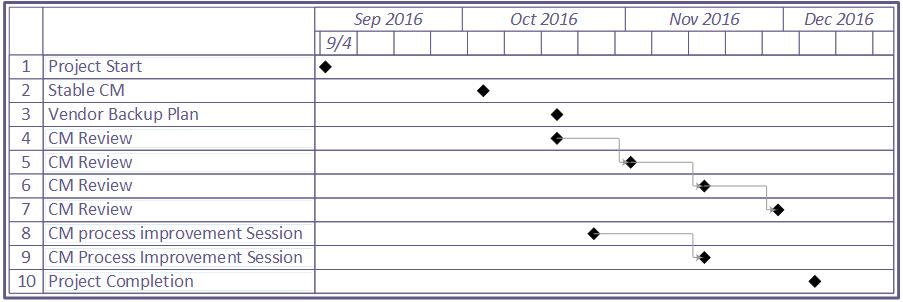
\includegraphics[scale=0.65]{CMSchedule}
 \caption{Confuguration Management Schedule}
 \label{fig:schedule}
\end{figure}

\subsection{SCM resources}
The configuration leader will require an estimated average of 2 hours a week to maintain the system configuration for the duration of the project.  Time spent on CM activities by other members of the team are not accounted for here.

\subsection{SCM plan maintenance}
Due to the importance of a stable SCM plan, all changes to this document must be approved by the configuration leader and the project manager.
\newline \newline
The configuration leader will do the following for the CM process improvement sessions:
\begin{itemize}
\item Review the effectiveness of this plan
\item Quantify losses due to defects in this plan
\item Review the effectiveness of GitHub and TortoiseGit
\item Investigate the literature for new CM methods, quantify the costs and benefits of improvements
\item Investigate new CM tools
\item Suggest specific improvements to this CM process
\item List the benefits of improvements
\end{itemize}

\newpage
\setcounter{secnumdepth}{0} 
\subsection{AnnexA: Configuration Management Tool Backup Plan}
The Configuration Leader will obtain and dedicate a USB flash drive for this project.  Once a week the Configuratin Leader will create a new clone of the current configuration of the project from GitHub on the USB drive.  All previous clone versions will be retained.  In the event of a failure or discontinunation of the GitHub service all requests to access files will be sent to the Configuration Leader.  Any changes will then be returned to the Configuration Leader for integration. 
\newpage
\subsection{Annex B: Bibliography}
Braude, Eric J., and Michael E. Bernstein. \textit{Software Engineering: Modern Approaches.} 2nd ed. Hoboken, NJ: J. Wiley \& Sons, 2011. Print.
\newline


\end{document}